\documentclass[UTF8,10pt]{ctexart}
\usepackage{amsmath, amssymb, geometry}
\usepackage{xcolor}
\usepackage{enumitem}
\usepackage{tcolorbox}
\usepackage{graphicx}
\usepackage{lastpage}
\usepackage{fancyhdr}

% Compact geometry
\geometry{a4paper, margin=1.5cm}

% Reduce paragraph spacing
\setlength{\parskip}{0pt}

% --- Custom Environments from Requirements ---
% 定义红色环境
\newenvironment{redenv}{\color{red}}{}

% 定义详细解析环境 (Compact version)
\newenvironment{detailedanalysis}{%
    \color{red}
    \begin{enumerate}[label=\textbf{第\arabic*步：}, leftmargin=*, align=left, itemsep=0pt, parsep=0pt, topsep=0pt, partopsep=0pt]
}{%
    \end{enumerate}
}

% 定义概念框 (Compact version)
\newenvironment{conceptbox}{%
    \begin{tcolorbox}[colback=red!5, colframe=red!50!black, title=概念解析, fonttitle=\bfseries, top=2pt, bottom=2pt, left=2pt, right=2pt]
}{%
    \end{tcolorbox}
}

% 定义公式推导环境 (Compact version)
\newenvironment{formuladerivation}{%
    \begin{enumerate}[label={\textbf{公式\arabic*：}}, leftmargin=*, align=left, itemsep=0pt, parsep=0pt]
}{%
    \end{enumerate}
}

% 定义题目和解析的分隔线 (With break hint)
\newcommand{\problemrule}{\par\filbreak\noindent\rule{\textwidth}{1.5pt}\vspace{-0.5em}}
\newcommand{\analysisrule}{\noindent\rule{\textwidth}{0.8pt}\vspace{-0.5em}}

% Choice Macros
\newcommand{\fourchoices}[4]{
    \par\noindent
    \begin{tabular*}{\linewidth}{@{\extracolsep{\fill}}llll}
        A.~#1 & B.~#2 & C.~#3 & D.~#4
    \end{tabular*}
}
\newcommand{\twochoices}[4]{
    \par\noindent
    \begin{tabular*}{\linewidth}{@{\extracolsep{\fill}}ll}
        A.~#1 & B.~#2 \\
        C.~#3 & D.~#4
    \end{tabular*}
}

\title{\textbf{周期测试讲义（详细解析版）}}
\author{自用上课讲义}
\date{\today}

\begin{document}
\small
\pagestyle{fancy}

\maketitle

% ==========================================================================================
% 第 I 卷 选择题
% ==========================================================================================
\section*{一、单项选择题}

% ========== 第1题 ==========
\problemrule
\section*{【题目1】函数的奇偶性}
函数 $f(x) = (e^x - e^{-x})\sin x$ 是 ( \quad )
\twochoices{偶函数}{奇函数}{非奇非偶函数}{无法判断}

\begin{redenv}
\analysisrule
\subsection*{逐步解析}

\begin{detailedanalysis}
\item \textbf{问题本质分析}
判断函数的奇偶性，核心在于比较 $f(-x)$ 与 $f(x)$ 的关系。
\begin{itemize}
    \item 若 $f(-x) = f(x)$，则为偶函数（图像关于 $y$ 轴对称）。
    \item 若 $f(-x) = -f(x)$，则为奇函数（图像关于原点对称）。
\end{itemize}

\item \textbf{详细求解过程}
\begin{enumerate}[label=(\alph*)]
    \item \textbf{代入 $-x$}：计算 $f(-x) = (e^{-x} - e^{-(-x)})\sin(-x)$。
    \item \textbf{化简表达式}：
    \begin{align*}
    f(-x) &= (e^{-x} - e^x)(-\sin x) \\
          &= -(e^x - e^{-x})(-\sin x) \quad \text{（提取负号）}\\
          &= (e^x - e^{-x})\sin x
    \end{align*}
    \item \textbf{比较结果}：发现 $f(-x) = f(x)$。
\end{enumerate}

\item \textbf{最终答案}
因为 $f(-x) = f(x)$，所以该函数是偶函数。故选 A。
\end{detailedanalysis}

\subsection*{核心公式与推导}
\begin{formuladerivation}
\item \textbf{常见函数的奇偶性}
\begin{itemize}
    \item 奇函数：$\sin x, \tan x, x^{2k-1}, e^x - e^{-x}, \ln \dfrac{1+x}{1-x}$
    \item 偶函数：$\cos x, x^{2k}, |x|, e^x + e^{-x}$
\end{itemize}
\item \textbf{奇偶运算口诀}
\begin{itemize}
    \item 奇 $\times$ 奇 = 偶
    \item 偶 $\times$ 偶 = 偶
    \item 奇 $\times$ 偶 = 奇
\end{itemize}
本题中，$g(x) = e^x - e^{-x}$ 是奇函数，$h(x) = \sin x$ 是奇函数，所以 $f(x) = g(x)h(x)$ 是偶函数。
\end{formuladerivation}

\subsection*{考点深度分析}
\begin{conceptbox}
\textbf{易错点}：
\begin{itemize}
    \item 忽略定义域的对称性（本题定义域为 $\mathbb{R}$，关于原点对称）。
    \item 符号计算错误，特别是在提取负号时。
\end{itemize}
\end{conceptbox}
\end{redenv}

% ========== 第2题 ==========
\problemrule
\section*{【题目2】等价无穷小}
当 $x \to 0$ 时，$1 - \cos 3x$ 与 $mx^2$ 是等价无穷小，则 $m$ 等于 ( \quad )
\fourchoices{$\dfrac{3}{2}$}{9}{$\dfrac{9}{2}$}{3}

\begin{redenv}
\analysisrule
\subsection*{逐步解析}

\begin{detailedanalysis}
\item \textbf{问题本质分析}
本题考查等价无穷小的概念。若 $\alpha \sim \beta$ ($x \to 0$)，则 $\lim\limits_{x\to 0} \dfrac{\alpha}{\beta} = 1$。
核心公式是 $1 - \cos \Box \sim \dfrac{1}{2}\Box^2$。

\item \textbf{详细求解过程}
\begin{enumerate}[label=(\alph*)]
    \item \textbf{应用公式}：当 $x \to 0$ 时，$3x \to 0$，故 $1 - \cos 3x \sim \dfrac{1}{2}(3x)^2$。
    \item \textbf{计算展开}：$\dfrac{1}{2}(3x)^2 = \dfrac{1}{2} \cdot 9x^2 = \dfrac{9}{2}x^2$。
    \item \textbf{建立方程}：题目已知 $1 - \cos 3x \sim mx^2$，由等价无穷小的传递性，$\dfrac{9}{2}x^2 = mx^2$。
    \item \textbf{求解}：$m = \dfrac{9}{2}$。
\end{enumerate}

\item \textbf{最终答案}
$m = \dfrac{9}{2}$。故选 C。
\end{detailedanalysis}

\subsection*{核心公式与推导}
\begin{formuladerivation}
\item \textbf{常用等价无穷小 ($x \to 0$)}
\begin{itemize}
    \item $1 - \cos x \sim \dfrac{1}{2}x^2$
    \item $\sin x \sim x, \quad \tan x \sim x, \quad \arcsin x \sim x, \quad \arctan x \sim x$
    \item $e^x - 1 \sim x, \quad \ln(1+x) \sim x$
    \item $(1+x)^\alpha - 1 \sim \alpha x$
\end{itemize}
\textbf{注意}：公式中的 $x$ 可以换成任何趋于 0 的表达式 $\Box$。
\end{formuladerivation}

\subsection*{考点深度分析}
\begin{conceptbox}
\textbf{易错点}：
\begin{itemize}
    \item \textbf{公式误用}：$1-\cos x \sim x^\dfrac{2}{2}$，常误记为 $x^2$。
    \item \textbf{系数遗漏}：在复合函数求导或等价代换时，容易遗漏内部函数的导数或系数（如本题中的 $3^2=9$）。
\end{itemize}
\textbf{解题技巧}：见到 $1-\cos \Box$ 立即想到 $\dfrac{1}{2}\Box^2$。
\end{conceptbox}
\end{redenv}

% ========== 第3题 ==========
\problemrule
\section*{【题目3】导数定义}
设 $f(x)$ 在点 $x_0$ 处可导，则 $\lim\limits_{\Delta x \to 0} \dfrac{f(x_0-\Delta x)-f(x_0)}{\Delta x} = $ ( \quad )
\fourchoices{$-f'(x_0)$}{$f'(-x_0)$}{$f'(x_0)$}{$f'(\Delta x)$}

\begin{redenv}
\analysisrule
\subsection*{逐步解析}

\begin{detailedanalysis}
\item \textbf{问题本质分析}
本题考查导数的极限定义形式：$f'(x_0) = \lim\limits_{h \to 0} \dfrac{f(x_0+h) - f(x_0)}{h}$。
关键在于凑成标准形式。

\item \textbf{详细求解过程}
\begin{enumerate}[label=(\alph*)]
    \item \textbf{观察极限式}：$\lim\limits_{\Delta x \to 0} \dfrac{f(x_0-\Delta x)-f(x_0)}{\Delta x}$。
    \item \textbf{变量代换}：令 $h = -\Delta x$。当 $\Delta x \to 0$ 时，$h \to 0$。
    \item \textbf{改写极限}：
    \[ \text{原式} = \lim\limits_{h \to 0} \dfrac{f(x_0+h)-f(x_0)}{-h} \]
    \item \textbf{提取常数}：
    \[ = -\lim\limits_{h \to 0} \dfrac{f(x_0+h)-f(x_0)}{h} \]
    \item \textbf{应用定义}：极限部分即为 $f'(x_0)$。
    \item \textbf{得出结果}：$-f'(x_0)$。
\end{enumerate}

\item \textbf{最终答案}
结果为 $-f'(x_0)$。故选 A。
\end{detailedanalysis}

\subsection*{考点深度分析}
\begin{conceptbox}
\textbf{易错点}：
\begin{itemize}
    \item \textbf{符号错误}：容易忽略分母中的 $\Delta x$ 与分子中变量变化量 $-\Delta x$ 的符号差异，直接选 C。
    \item \textbf{形式混淆}：容易混淆 $f'(-x_0)$ 和 $-f'(x_0)$。
\end{itemize}
\textbf{核心考点}：导数定义的本质是极限，需熟练掌握其多种变体形式，如 $\lim\limits_{\Delta x \to 0} \dfrac{f(x_0+a\Delta x) - f(x_0)}{b\Delta x} = \dfrac{a}{b}f'(x_0)$。
\end{conceptbox}
\end{redenv}

% ========== 第4题 ==========
\problemrule
\section*{【题目4】拐点判定}
设函数 $y = f(x)$ 在区间 $(0,2)$ 内具有二阶导数，若 $x \in (0,1)$ 时，$f''(x) < 0$，$x \in (1,2)$ 时，$f''(x) > 0$，则 ( \quad )
\begin{enumerate}[label=\Alph*.]
    \item $f(1)$ 是函数 $f(x)$ 的极大值
    \item 点 $(1, f(1))$ 是曲线 $y = f(x)$ 的拐点
    \item $f(1)$ 是函数 $f(x)$ 的极小值
    \item 点 $(1, f(1))$ 不是曲线 $y = f(x)$ 的拐点
\end{enumerate}

\begin{redenv}
\analysisrule
\subsection*{逐步解析}

\begin{detailedanalysis}
\item \textbf{问题本质分析}
二阶导数 $f''(x)$ 的符号决定曲线的凹凸性：
\begin{itemize}
    \item $f''(x) > 0 \implies$ 凹（下凸）。
    \item $f''(x) < 0 \implies$ 凸（上凸）。
\end{itemize}
拐点是曲线凹凸性发生改变的点。

\item \textbf{详细求解过程}
\begin{enumerate}[label=(\alph*)]
    \item \textbf{分析 $(0,1)$ 区间}：$f''(x) < 0$，曲线是凸的。
    \item \textbf{分析 $(1,2)$ 区间}：$f''(x) > 0$，曲线是凹的。
    \item \textbf{分析 $x=1$ 处}：在 $x=1$ 左右两侧，二阶导数符号由负变正，凹凸性发生了改变。
    \item \textbf{结论}：点 $(1, f(1))$ 是曲线的拐点。
\end{enumerate}
注意：极值点通常由一阶导数 $f'(x)$ 的变号点决定，二阶导数无法直接判定极值（除非结合二阶导数判别法，但前提是 $f'(1)=0$）。

\item \textbf{最终答案}
点 $(1, f(1))$ 是曲线 $y = f(x)$ 的拐点。故选 B。
\end{detailedanalysis}

\subsection*{考点深度分析}
\begin{conceptbox}
\textbf{核心考点}：
\begin{itemize}
    \item \textbf{二阶导数与凹凸性}：$f'' > 0$ 凹，$f'' < 0$ 凸。
    \item \textbf{拐点}：二阶导数变号的点（连续曲线上）。
\end{itemize}
\textbf{易错点}：
\begin{itemize}
    \item 混淆极值点与拐点：极值点看一阶导数，$f'(x)=0$；拐点看二阶导数，$f''(x)=0$ 或不存在。
    \item $f''(x_0)=0$ 并不一定是拐点，必须检查两侧符号是否改变（如同 $f'(x_0)=0$ 不一定是极值点）。
\end{itemize}
\end{conceptbox}
\end{redenv}

% ========== 第5题 ==========
\problemrule
\section*{【题目5】渐近线}
曲线 $y = \dfrac{x^2}{x^2+x-2}$ 的水平渐近线为 ( \quad )
\fourchoices{$y=1$}{$y=0$}{$x=-2$}{$x=1$}

\begin{redenv}
\analysisrule
\subsection*{逐步解析}

\begin{detailedanalysis}
\item \textbf{问题本质分析}
\begin{itemize}
    \item \textbf{水平渐近线}：看 $x \to \infty$ 时的极限 $\lim\limits_{x\to \infty} f(x) = A$。
    \item \textbf{铅直渐近线}：看分母为零的点。
\end{itemize}

\item \textbf{详细求解过程}
\begin{enumerate}[label=(\alph*)]
    \item \textbf{求极限}：
    \[ \lim\limits_{x \to \infty} \dfrac{x^2}{x^2+x-2} \]
    \item \textbf{抓大头}：分子分母同除以最高次幂 $x^2$。
    \[ = \lim\limits_{x \to \infty} \dfrac{1}{1 + \dfrac{1}{x} - \dfrac{2}{x^2}} = \dfrac{1}{1+0-0} = 1 \]
    \item \textbf{结论}：水平渐近线为 $y=1$。
\end{enumerate}
注：若求铅直渐近线，令 $x^2+x-2=(x+2)(x-1)=0$，得 $x=-2$ 和 $x=1$。

\item \textbf{最终答案}
水平渐近线为 $y=1$。故选 A。
\end{detailedanalysis}

\subsection*{考点深度分析}
\begin{conceptbox}
\textbf{核心考点}：
\begin{itemize}
    \item \textbf{水平渐近线}：$x \to \infty$ 时，$y \to A$。
    \item \textbf{铅直渐近线}：$x \to x_0$ 时，$y \to \infty$（通常是分母为零的点）。
\end{itemize}
\textbf{技巧}：对于有理分式 $\dfrac{P(x)}{Q(x)}$，若分子分母同次，水平渐近线为最高次系数之比。本题 $\dfrac{1}{1}=1$。
\end{conceptbox}
\end{redenv}

% ========== 第6题 ==========
\problemrule
\section*{【题目6】定积分应用（面积）}
若曲线 $y = \sqrt{x}$ 与 $y = kx$ 所围平面图形的面积为 $\dfrac{1}{6}$，则 $k = $ ( \quad )
\fourchoices{1}{0}{-2}{2}

\begin{redenv}
\analysisrule
\subsection*{逐步解析}

\begin{detailedanalysis}
\item \textbf{问题本质分析}
计算两条曲线围成的面积，需先确定交点，再利用定积分求解。
题目隐含 $k>0$，因为若 $k \le 0$，在 $x \ge 0$ 时两曲线无封闭区域（$y=\sqrt{x} \ge 0$）。

\item \textbf{详细求解过程}
\begin{enumerate}[label=(\alph*)]
    \item \textbf{第一步：求交点}
    联立方程 $\sqrt{x} = kx$，两边平方得 $x = k^2 x^2$。
    移项整理：$k^2 x^2 - x = 0 \implies x(k^2 x - 1) = 0$。
    解得交点横坐标：$x_1 = 0, \quad x_2 = \dfrac{1}{k^2}$。

    \item \textbf{第二步：列积分式}
    在区间 $[0, \dfrac{1}{k^2}]$ 上，比较 $\sqrt{x}$ 与 $kx$ 的大小。
    （可取特殊值验证：例如令 $k=1$，则 $x \in [0,1]$，$\sqrt{x} \ge x$）。
    故面积公式为：
    \[ S = \int_0^{\dfrac{1}{k^2}} (\sqrt{x} - kx) \, dx \]

    \item \textbf{第三步：计算积分（详细步骤）}
    \begin{align*}
    S &= \left[ \dfrac{2}{3}x^{\dfrac{3}{2}} - \dfrac{k}{2}x^2 \right]_0^{\dfrac{1}{k^2}} \\
      &= \left( \dfrac{2}{3} \cdot \left(\dfrac{1}{k^2}\right)^{\dfrac{3}{2}} - \dfrac{k}{2} \cdot \left(\dfrac{1}{k^2}\right)^2 \right) - 0 \\
      &= \dfrac{2}{3} \cdot \dfrac{1}{(k^2)^{\dfrac{3}{2}}} - \dfrac{k}{2} \cdot \dfrac{1}{k^4} \\
      &= \dfrac{2}{3} \cdot \dfrac{1}{k^3} - \dfrac{1}{2k^3} \\
      &= \dfrac{4}{6k^3} - \dfrac{3}{6k^3} \quad (\text{通分，公分母为 } 6k^3) \\
      &= \dfrac{1}{6k^3}
    \end{align*}

    \item \textbf{第四步：解方程求 k}
    由题意 $S = \dfrac{1}{6}$，即：
    \[ \dfrac{1}{6k^3} = \dfrac{1}{6} \implies k^3 = 1 \implies k = 1 \]
\end{enumerate}

\item \textbf{最终答案}
$k=1$。故选 A。
\end{detailedanalysis}

\subsection*{考点深度分析}
\begin{conceptbox}
\textbf{核心考点}：
\begin{itemize}
    \item \textbf{定积分几何意义}：面积。
    \item \textbf{微元法}：$dS = |f(x) - g(x)|\, dx$。
\end{itemize}
\textbf{定积分定义通俗讲解（四步曲）}：
定积分 $\int_a^b f(x)\, dx$ 的本质是求和的极限。想象我们要计算曲边梯形的面积，可以分为四个步骤：
\begin{enumerate}
    \item \textbf{分割}：把区间 $[a, b]$ 切成 $n$ 个小段（就像把原本不规则的图形切成很多细细的竖条）。
    \item \textbf{近似}：在每一小段上任取一点 $\xi_i$，用高为 $f(\xi_i)$ 的矩形面积近似代替该小段的曲边梯形面积（“以直代曲”）。
    \item \textbf{求和}：把所有小矩形的面积加起来，得到总面积的近似值 $\sum\limits_{i=1}^n f(\xi_i) \Delta x_i$。
    \item \textbf{取极限}：当切分得足够细（最大小段长度 $\lambda \to 0$）时，这个和式的极限就是定积分的值（精确面积）。
\end{enumerate}
\begin{center}
    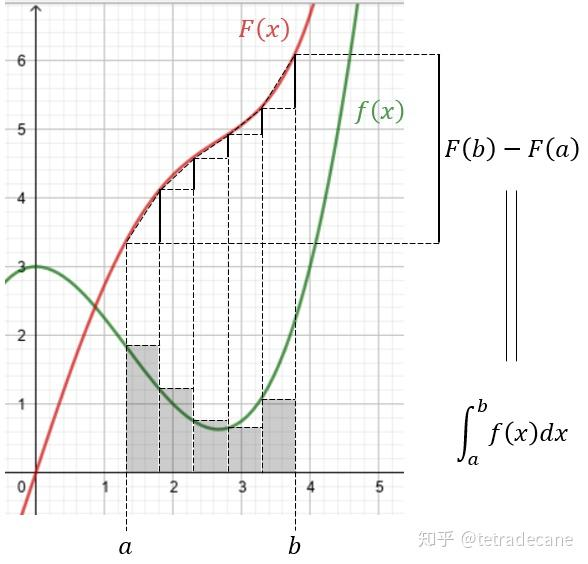
\includegraphics[width=0.4\textwidth]{定积分定义.png} \\
    \small{\textit{图示：通过矩形面积和（黎曼和-定积分定义）逼近曲边梯形面积}}
\end{center}
即：$\lim\limits_{\lambda \to 0} \sum\limits_{i=1}^n f(\xi_i) \Delta x_i = \int_a^b f(x)\, dx$。

\textbf{易错点}：
\begin{itemize}
    \item 积分上下限弄反或计算错误。
    \item 忽略两曲线位置关系（谁在上方），导致面积为负（面积恒为正）。
\end{itemize}
\end{conceptbox}
\end{redenv}

% ========== 第7题 ==========
\problemrule
\section*{【题目7】连续性与可导性}
$f(x) = \begin{cases} x\sin\dfrac{1}{x}, & x \neq 0 \\ 0, & x=0 \end{cases}$，在 $x=0$ 处 ( \quad )
\twochoices{极限不存在}{极限存在但不连续}{连续但不可导}{可导但不连续}

\begin{redenv}
\analysisrule
\subsection*{逐步解析}

\begin{detailedanalysis}
\item \textbf{问题本质分析}
考查分段函数在分界点的连续性和可导性。
\begin{itemize}
    \item \textbf{连续性}：$\lim\limits_{x\to 0} f(x) = f(0)$。
    \item \textbf{可导性}：$\lim\limits_{x\to 0} \dfrac{f(x)-f(0)}{x-0}$ 存在。
\end{itemize}

\item \textbf{详细求解过程}
\begin{enumerate}[label=(\alph*)]
    \item \textbf{判断连续性}：
    \[ \lim\limits_{x\to 0} x\sin\dfrac{1}{x} = 0 \quad (\text{无穷小} \times \text{有界量} = \text{无穷小}) \]
    因为 $\lim\limits_{x\to 0} f(x) = 0 = f(0)$，所以函数在 $x=0$ 处\textbf{连续}。
    \item \textbf{判断可导性}：
    \[ f'(0) = \lim\limits_{x\to 0} \dfrac{f(x)-f(0)}{x-0} = \lim\limits_{x\to 0} \dfrac{x\sin\dfrac{1}{x} - 0}{x} = \lim\limits_{x\to 0} \sin\dfrac{1}{x} \]
    当 $x \to 0$ 时，$\dfrac{1}{x} \to \infty$，$\sin\dfrac{1}{x}$ 在 $[-1, 1]$ 之间振荡，极限不存在。
    所以函数在 $x=0$ 处\textbf{不可导}。
\end{enumerate}

\item \textbf{最终答案}
连续但不可导。故选 C。
\end{detailedanalysis}

\subsection*{考点深度分析}
\begin{conceptbox}
\textbf{核心考点}：
\begin{itemize}
    \item \textbf{分段函数}：分界点处的连续与可导性是必考点。
    \item \textbf{振荡间断点}：$\sin(\dfrac{1}{x})$ 在 $x \to 0$ 时振荡，极限不存在。
\end{itemize}
\textbf{结论记忆}：$x^k \sin(\dfrac{1}{x})$ 在 $x \to 0$ 时：
\begin{itemize}
    \item $k=0$：极限不存在（振荡）。
    \item $k=1$：连续但不可导。
    \item $k=2$：连续且可导（导函数连续性需进一步判断）。
\end{itemize}
\end{conceptbox}
\end{redenv}

% ========== 第8题 ==========
\problemrule
\section*{【题目8】定积分性质}
设常数 $a > 0$, 则 $\int_{-a}^{a} (x^2 + x\sqrt{a^2-x^2})dx = $ ( \quad )
\fourchoices{0}{$a^3$}{$\dfrac{2}{3}a^3$}{$\dfrac{2}{3}\pi a^3$}

\begin{redenv}
\analysisrule
\subsection*{逐步解析}

\begin{detailedanalysis}
\item \textbf{问题本质分析}
对称区间 $[-a, a]$ 上的定积分，利用奇偶性简化计算。
\begin{itemize}
    \item $\int_{-a}^a \text{奇函数} \, dx = 0$
    \item $\int_{-a}^a \text{偶函数} \, dx = 2\int_0^a \text{偶函数} \, dx$
\end{itemize}

\item \textbf{详细求解过程}
\begin{enumerate}[label=(\alph*)]
    \item \textbf{拆分积分}：
    \[ I = \int_{-a}^a x^2 \, dx + \int_{-a}^a x\sqrt{a^2-x^2} \, dx \]
    \item \textbf{判断奇偶性}：
    \begin{itemize}
        \item $f_1(x) = x^2$ 是偶函数。
        \item $f_2(x) = x\sqrt{a^2-x^2}$，因为 $f_2(-x) = (-x)\sqrt{a^2-(-x)^2} = -x\sqrt{a^2-x^2} = -f_2(x)$，是奇函数。
    \end{itemize}
    \item \textbf{计算积分}：
    \begin{itemize}
        \item $\int_{-a}^a x\sqrt{a^2-x^2} \, dx = 0$。
        \item $\int_{-a}^a x^2 \, dx = 2\int_0^a x^2 \, dx = 2 \left[ \dfrac{1}{3}x^3 \right]_0^a = \dfrac{2}{3}a^3$。
    \end{itemize}
\end{enumerate}

\item \textbf{最终答案}
$\dfrac{2}{3}a^3$。故选 C。
\end{detailedanalysis}

\subsection*{考点深度分析}
\begin{conceptbox}
\textbf{核心考点}：
\begin{itemize}
    \item \textbf{对称区间积分}：$\int_{-a}^a f(x)\, dx$。
    \item \textbf{奇偶性判断}：$f(-x) = -f(x)$ 为奇函数，$f(-x) = f(x)$ 为偶函数。
\end{itemize}
\textbf{技巧}：见到对称区间，首先考虑奇偶性，可以大大简化计算。不用死算。
\end{conceptbox}
\end{redenv}

% ========== 第9题 ==========
\problemrule
\section*{【题目9】高阶导数}
设函数 $y = x^n + a_1 x^{n-1} + \cdots + a_n$，则 $y^{(n)} = $ ( \quad )
\fourchoices{$a_n$}{$n!$}{0}{$n!a_n$}

\begin{redenv}
\analysisrule
\subsection*{逐步解析}

\begin{detailedanalysis}
\item \textbf{问题本质分析}
幂函数 $x^k$ 的高阶导数规律。
若 $k < n$，则 $(x^k)^{(n)} = 0$。
若 $k = n$，则 $(x^n)^{(n)} = n!$。

\item \textbf{详细求解过程}
\begin{enumerate}[label=(\alph*)]
    \item \textbf{逐项求导}：
    $y$ 是一个 $n$ 次多项式，最高次项为 $x^n$。
    \item \textbf{应用规律}：
    \begin{itemize}
        \item $(x^n)^{(n)} = n(n-1)\cdots 1 = n!$
        \item $(a_1 x^{n-1})^{(n)} = 0$ （次数小于求导阶数）
        \item 其他低次项的 $n$ 阶导数均为 0。
    \end{itemize}
    \item \textbf{求和}：$y^{(n)} = n! + 0 + \cdots + 0 = n!$。
\end{enumerate}

\item \textbf{最终答案}
$n!$。故选 B。
\end{detailedanalysis}

\subsection*{考点深度分析}
\begin{conceptbox}
\textbf{核心考点}：
\begin{itemize}
    \item \textbf{高阶导数}：$(x^n)^{(n)} = n!$，$(e^{kx})^{(n)} = k^n e^{kx}$。
    \item \textbf{线性性质}：$(u+v)^{(n)} = u^{(n)} + v^{(n)}$。
\end{itemize}
\textbf{易错点}：
\begin{itemize}
    \item 混淆阶乘与幂次。
    \item 认为低次项的高阶导数即为自身（实际上是0）。
\end{itemize}
\end{conceptbox}
\end{redenv}

% ========== 第10题 ==========
\problemrule
\section*{【题目10】级数收敛性}
若级数 $\sum\limits_{n=1}^{\infty} (u_{2n-1} + u_{2n})$ 收敛，则 ( \quad )
\twochoices{$\sum\limits_{n=1}^{\infty} u_{2n}$ 必收敛}{$\sum\limits_{n=1}^{\infty} u_n$ 未必收敛}{ $\lim\limits_{n \to \infty} u_n = 0$}{$\sum\limits_{n=1}^{\infty} u_n$ 发散}

\begin{redenv}
\analysisrule
\subsection*{逐步解析}

\begin{detailedanalysis}
\item \textbf{问题本质分析}
级数加括号后的收敛性与原级数收敛性的关系。
若原级数收敛，加括号后必收敛且和不变。
\textbf{反之不成立}。

\item \textbf{详细求解过程}
\begin{enumerate}[label=(\alph*)]
    \item \textbf{举反例}：
    设 $u_n = (-1)^{n-1}$，即 $1, -1, 1, -1, \dots$。
    \item \textbf{验证条件}：
    $\sum (u_{2n-1} + u_{2n}) = (1-1) + (1-1) + \dots = 0 + 0 + \dots = 0$，收敛。
    \item \textbf{验证选项}：
    \begin{itemize}
        \item $\sum u_n = 1-1+1-1\dots$ 发散。所以 A、D 不一定（本例发散，但若 $u_n=0$ 则收敛）。
        \item $\lim u_n$ 不存在，不为 0。排除 C。
        \item $\sum u_n$ 未必收敛（可能发散，也可能收敛）。
    \end{itemize}
\end{enumerate}

\item \textbf{最终答案}
$\sum\limits_{n=1}^{\infty} u_n$ 未必收敛。故选 B。
\end{detailedanalysis}

\subsection*{考点深度分析}
\begin{conceptbox}
\textbf{核心考点}：
\begin{itemize}
    \item \textbf{收敛级数性质}：若 $\sum u_n, \sum v_n$ 收敛，则 $\sum (u_n \pm v_n)$ 收敛。
    \item \textbf{加括号性质}：收敛级数加括号后仍收敛且和不变。发散级数加括号后可能收敛。
\end{itemize}
\textbf{易错点}：
\begin{itemize}
    \item 误以为加括号不改变敛散性（仅对收敛级数成立）。
    \item 误以为 $\lim u_n = 0$ 是级数收敛的充分条件（其实是必要条件）。
\end{itemize}
\end{conceptbox}
\end{redenv}

% ========== 第11题 ==========
\problemrule
\section*{【题目11】微分方程反求}
下列微分方程中，通解为 $y = C_1e^{2x} + C_2e^{3x}$ 的二阶常系数齐次线性微分方程是 ( \quad )
\twochoices{$y'' - 5y' + 6y = 0$}{$y'' + 5y' + 6y = 0$}{$y'' - 6y' + 5y = 0$}{$y'' + 6y' + 5y = 0$}

\begin{redenv}
\analysisrule
\subsection*{逐步解析}

\begin{detailedanalysis}
\item \textbf{问题本质分析}
由通解形式 $y = C_1 e^{r_1 x} + C_2 e^{r_2 x}$ 反推特征方程 $(r-r_1)(r-r_2)=0$，进而得到微分方程 $y'' - (r_1+r_2)y' + r_1r_2 y = 0$。

\item \textbf{详细求解过程}
\begin{enumerate}[label=(\alph*)]
    \item \textbf{识别特征根}：由通解形式可知，特征根为 $r_1=2, r_2=3$。
    \item \textbf{构造特征方程}：
    \[ (r-2)(r-3) = 0 \implies r^2 - 5r + 6 = 0 \]
    \item \textbf{对应微分方程}：
    \[ y'' - 5y' + 6y = 0 \]
\end{enumerate}

\item \textbf{最终答案}
$y'' - 5y' + 6y = 0$。故选 A。（注：题目选项与推导一致）
\end{detailedanalysis}

\subsection*{考点深度分析}
\begin{conceptbox}
\textbf{核心考点}：
\begin{itemize}
    \item \textbf{二阶常系数齐次线性微分方程}：通解结构与特征根的关系。
    \item \textbf{韦达定理}：对于 $y''+py'+qy=0$，有 $r_1+r_2 = -p, \quad r_1 \cdot r_2 = q$。
    \item \textbf{基础补充}：
    \begin{itemize}
        \item \textbf{求根公式}：$ax^2+bx+c=0 \implies x_{1,2} = \dfrac{-b \pm \sqrt{b^2-4ac}}{2a}$。
        \item \textbf{高中韦达定理}：$x_1+x_2 = -\dfrac{b}{a}, \quad x_1 x_2 = \dfrac{c}{a}$。
    \end{itemize}
\end{itemize}
\textbf{易错点}：
\begin{itemize}
    \item 符号错误：方程 $y''+py'+qy=0$ 对应 $r^2+pr+q=0$。注意 $p = -(r_1+r_2)$。
\end{itemize}
\end{conceptbox}
\end{redenv}

% ========== 第12题 ==========
\problemrule
\section*{【题目12】变限积分求导}
$\dfrac{d}{dx} \int_a^b \cos t \, dt = $ ( \quad )
\twochoices{$\cos b - \cos a$}{0}{$\sin b - \sin a$}{$\sin a - \sin b$}

\begin{redenv}
\analysisrule
\subsection*{逐步解析}

\begin{detailedanalysis}
\item \textbf{问题本质分析}
区分\textbf{定积分}与\textbf{变限积分}。
$\int_a^b f(t)\, dt$ 是一个常数（若 $a,b$ 为常数）。
常数的导数为 0。

\item \textbf{详细求解过程}
\begin{enumerate}[label=(\alph*)]
    \item \textbf{观察积分}：积分通过 $\int_a^b$ 定义，上下限均为常数。
    \item \textbf{判断类型}：这是一个定积分，其结果是一个具体的数值（常数）。
    \item \textbf{求导运算}：常数的导数为 0。
    \[ \dfrac{d}{dx} (\text{常数}) = 0 \]
\end{enumerate}

\item \textbf{最终答案}
0。故选 B。
\end{detailedanalysis}

\subsection*{考点深度分析}
\begin{conceptbox}
\textbf{核心考点}：
\begin{itemize}
    \item \textbf{变限积分求导}：$\dfrac{d}{dx} \int_a^x f(t)\, dt = f(x)$。
    \item \textbf{定积分}：$\int_a^b f(t)\, dt$ 是常数。
\end{itemize}
\textbf{易错点}：
\begin{itemize}
    \item 看到积分号就想求导得到被积函数，忽略了积分上限是常数还是变量。
    \item 计算常数导数时忘记为0。
\end{itemize}
\end{conceptbox}
\end{redenv}

% ==========================================================================================
% 第 II 卷 非选择题
% ==========================================================================================
\section*{二、填空题}

% ========== 第13题 ==========
\problemrule
\section*{【题目13】微分计算}
设函数 $f(x) = \sqrt{x+x^2}$，则 $df(x)|_{x=1} = $\underline{\hspace{4cm}}.

\begin{redenv}
\analysisrule
\subsection*{逐步解析}

\begin{detailedanalysis}
\item \textbf{问题本质分析}
计算函数在某点的微分。公式：$dy = f'(x_0)\, dx$。
核心在于求导 $f'(x)$ 并代入 $x=1$。

\item \textbf{详细求解过程}
\begin{enumerate}[label=(\alph*)]
    \item \textbf{求导数} $f'(x)$：
    \[ f(x) = (x+x^2)^{\dfrac{1}{2}} \]
    \[ f'(x) = \dfrac{1}{2}(x+x^2)^{-\dfrac{1}{2}} \cdot (1+2x) = \dfrac{1+2x}{2\sqrt{x+x^2}} \]
    \item \textbf{计算值} $f'(1)$：
    \[ f'(1) = \dfrac{1+2(1)}{2\sqrt{1+1^2}} = \dfrac{3}{2\sqrt{2}} = \dfrac{3\sqrt{2}}{4} \]
    \item \textbf{写出微分}：
    \[ df|_{x=1} = f'(1)\, dx = \dfrac{3\sqrt{2}}{4}\, dx \]
\end{enumerate}

\item \textbf{最终答案}
$\dfrac{3\sqrt{2}}{4}\, dx$
\end{detailedanalysis}

\subsection*{考点深度分析}
\begin{conceptbox}
\textbf{核心考点}：
\begin{itemize}
    \item \textbf{微分定义}：$dy = y'\, dx$。
    \item \textbf{导数计算}：复合函数求导法则。
\end{itemize}
\textbf{易错点}：
\begin{itemize}
    \item \textbf{格式错误}：填空题求微分，结果必须带 $dx$。只写导数值 $f'(x_0)$ 是错误的。
    \item 根式求导时系数容易出错。
\end{itemize}
\end{conceptbox}
\end{redenv}

% ========== 第14题 ==========
\problemrule
\section*{【题目14】空间直线夹角}
直线 $\dfrac{x-1}{1} = \dfrac{y}{-4} = \dfrac{z+3}{1}$ 和直线 $\dfrac{x}{2} = \dfrac{y+2}{-2} = \dfrac{z}{-1}$ 的夹角为\underline{\hspace{4cm}}.

\begin{redenv}
\analysisrule
\subsection*{逐步解析}

\begin{detailedanalysis}
\item \textbf{问题本质分析}
两条直线的夹角 $\theta$ 由其方向向量 $\vec{s_1}, \vec{s_2}$ 决定。
公式：$\cos \theta = \dfrac{|\vec{s_1} \cdot \vec{s_2}|}{|\vec{s_1}| |\vec{s_2}|}$。

\item \textbf{详细求解过程}
\begin{enumerate}[label=(\alph*)]
    \item \textbf{确定方向向量}：
    \[ \vec{s_1} = (1, -4, 1), \quad \vec{s_2} = (2, -2, -1) \]
    \item \textbf{计算数量积}：
    \[ \vec{s_1} \cdot \vec{s_2} = 1\times 2 + (-4)\times (-2) + 1\times (-1) = 2 + 8 - 1 = 9 \]
    \item \textbf{计算模长}：
    \[ |\vec{s_1}| = \sqrt{1^2 + (-4)^2 + 1^2} = \sqrt{18} = 3\sqrt{2} \]
    \[ |\vec{s_2}| = \sqrt{2^2 + (-2)^2 + (-1)^2} = \sqrt{9} = 3 \]
    \item \textbf{计算余弦值}：
    \[ \cos \theta = \dfrac{|9|}{3\sqrt{2} \cdot 3} = \dfrac{9}{9\sqrt{2}} = \dfrac{1}{\sqrt{2}} = \dfrac{\sqrt{2}}{2} \]
    \item \textbf{确定角度}：
    $\theta = \arccos \dfrac{\sqrt{2}}{2} = \dfrac{\pi}{4}$。
\end{enumerate}

\item \textbf{最终答案}
$\dfrac{\pi}{4}$ （或 $45^\circ$）
\end{detailedanalysis}

\subsection*{考点深度分析}
\begin{conceptbox}
\textbf{核心考点}：
\begin{itemize}
    \item \textbf{空间解析几何}：直线的方向向量。
    \item \textbf{夹角公式}：利用数量积求夹角。
\end{itemize}
\textbf{易错点}：
\begin{itemize}
    \item 方向向量提取错误，特别是分母位置（需化为标准式 $\dfrac{x-x_0}{m} = \dfrac{y-y_0}{n} = \dfrac{z-z_0}{p}$）。
\end{itemize}
\end{conceptbox}
\end{redenv}

% ========== 第15题 ==========
\problemrule
\section*{【题目15】隐函数求切线/法线}
设 $y = f(x)$ 由方程 $e^{2x+y} - \cos(xy) = e - 1$ 所确定，则曲线 $y = f(x)$ 在点 $(0,1)$ 处的法线方程为\underline{\hspace{4cm}}.

\begin{redenv}
\analysisrule
\subsection*{逐步解析}

\begin{detailedanalysis}
\item \textbf{问题本质分析}
\begin{itemize}
    \item 隐函数求导求 $y'$。
    \item 切线斜率 $k_t = y'|_{x_0}$。
    \item 法线斜率 $k_n = -\dfrac{1}{k}_t$。
    \item 点斜式写方程。
\end{itemize}

\item \textbf{详细求解过程}
\begin{enumerate}[label=(\alph*)]
    \item \textbf{方程两边求导}：
    \[ \dfrac{d}{dx}(e^{2x+y}) - \dfrac{d}{dx}(\cos(xy)) = 0 \]
    \[ e^{2x+y}(2+y') - (-\sin(xy))(y + xy') = 0 \]
    \[ e^{2x+y}(2+y') + \sin(xy)(y + xy') = 0 \]
    \item \textbf{代入点 $(0,1)$}：
    \[ e^{0+1}(2+y'(0)) + \sin(0)(1 + 0) = 0 \]
    \[ e(2+y'(0)) + 0 = 0 \]
    由于 $e \neq 0$，故 $2 + y'(0) = 0 \implies y'(0) = -2$。
    \item \textbf{求法线斜率}：
    \[ k_{normal} = -\dfrac{1}{y'(0)} = -\dfrac{1}{-2} = \dfrac{1}{2} \]
    \item \textbf{写出法线方程}：
    \[ y - 1 = \dfrac{1}{2}(x - 0) \implies y = \dfrac{1}{2}x + 1 \quad \text{或} \quad x - 2y + 2 = 0 \]
\end{enumerate}

\item \textbf{最终答案}
$x - 2y + 2 = 0$ （或 $y=\dfrac{1}{2}x+1$）
\end{detailedanalysis}

\subsection*{考点深度分析}
\begin{conceptbox}
\textbf{核心考点}：
\begin{itemize}
    \item \textbf{隐函数求导}：方程两边对 $x$ 求导，视 $y$ 为 $x$ 的函数。
    \item \textbf{法线斜率}：$k_n = -\dfrac{1}{y}'$。
\end{itemize}
\textbf{易错点}：
\begin{itemize}
    \item 求导时漏乘 $y'$（链式法则）。
    \item 混淆切线与法线，导致斜率用反。
\end{itemize}
\end{conceptbox}
\end{redenv}

% ========== 第16题 ==========
\problemrule
\section*{【题目16】幂级数收敛区间}
设 $\sum\limits_{n=1}^{\infty} a_n x^n$ 的收敛半径为 3，则 $\sum\limits_{n=1}^{\infty} n a_n (x-1)^{n-1}$ 的收敛区间为\underline{\hspace{4cm}}.

\begin{redenv}
\analysisrule
\subsection*{逐步解析}

\begin{detailedanalysis}
\item \textbf{问题本质分析}
\begin{itemize}
    \item 幂级数逐项求导后收敛半径 $R$ 不变。
    \item 级数中心平移：$x^n \to (x-x_0)^n$。
    \item 收敛区间 = $(x_0-R, x_0+R)$。
\end{itemize}

\item \textbf{详细求解过程}
\begin{enumerate}[label=(\alph*)]
    \item \textbf{分析原级数}：
    $\sum a_n x^n$ 的收敛半径 $R=3$。
    \item \textbf{分析新级数}：
    $\sum n a_n (x-1)^{n-1}$ 是级数 $\sum a_n (x-1)^n$ 的导数级数。
    \begin{itemize}
        \item 平移：$x \to x-1$，中心变为 $x_0=1$。
        \item 求导：收敛半径保持不变，仍为 $R=3$。
    \end{itemize}
    \item \textbf{确定开区间}：
    $|x-1| < 3 \implies -3 < x-1 < 3 \implies -2 < x < 4$。
    \item \textbf{端点说明}：
     逐项求导后的级数在端点的收敛性可能会改变（通常变差），且题目未给出 $a_n$ 具体形式，无法确定端点是否收敛。按照惯例，若无更多信息，通常填写开区间。
\end{enumerate}

\item \textbf{最终答案}
$(-2, 4)$
\end{detailedanalysis}

\subsection*{考点深度分析}
\begin{conceptbox}
\textbf{核心考点}：
\begin{itemize}
    \item \textbf{幂级数求导}：收敛半径 $R$ 不变。
    \item \textbf{收敛区间}：$(x_0-R, x_0+R)$。
\end{itemize}
\textbf{易错点}：
\begin{itemize}
    \item 端点收敛性可能改变，除非题目有特殊说明，否则一般变为开区间或保持原状（视具体级数而定），填空题通常填开区间较为稳妥，除非明确知道端点情况。
\end{itemize}
\end{conceptbox}
\end{redenv}

% ==========================================================================================
% 第 III 卷 计算题
% ==========================================================================================
\newpage
\section*{三、计算题}

% ========== 第17题 ==========
\problemrule
\section*{【题目17】极限计算}
求极限 $\lim\limits_{x \to 0} \dfrac{\sqrt{2} - \sqrt{1 + \cos 2x}}{\sin^2 2x}$.

\begin{redenv}
\analysisrule
\subsection*{逐步解析}

\begin{detailedanalysis}
\item \textbf{问题本质分析}
\begin{itemize}
    \item 类型：$\dfrac{0}{0}$ 型不定式。
    \item 关键变形：三角恒等式 $1+\cos 2x = 2\cos^2 x$ 和等价无穷小。
\end{itemize}

\item \textbf{解法一：三角恒等变换（提取公因式）}
\begin{enumerate}[label=(\alph*)]
    \item \textbf{分子变形}：
    \[ \sqrt{1+\cos 2x} = \sqrt{2\cos^2 x} = \sqrt{2}|\cos x| \]
    因为 $x \to 0$，$\cos x > 0$，所以 $|\cos x| = \cos x$。
    分子 $\sqrt{2} - \sqrt{2}\cos x = \sqrt{2}(1 - \cos x)$。
    \item \textbf{等价无穷小代换}：
    \begin{itemize}
        \item 分子：$1 - \cos x \sim \dfrac{1}{2}x^2$，所以分子 $\sim \sqrt{2} \cdot \dfrac{1}{2}x^2$。
        \item 分母：$\sin 2x \sim 2x$，所以 $\sin^2 2x \sim (2x)^2 = 4x^2$。
    \end{itemize}
    \item \textbf{计算极限}：
    \[ \lim\limits_{x \to 0} \dfrac{\dfrac{\sqrt{2}}{2}x^2}{4x^2} = \dfrac{\sqrt{2}}{8} \]
\end{enumerate}

\item \textbf{解法二：分子有理化（利用平方差公式）}
\begin{enumerate}[label=(\alph*)]
    \item \textbf{分子有理化}：
    \[ \text{原式} = \lim\limits_{x \to 0} \dfrac{(\sqrt{2} - \sqrt{1 + \cos 2x})(\sqrt{2} + \sqrt{1 + \cos 2x})}{\sin^2 2x (\sqrt{2} + \sqrt{1 + \cos 2x})} \]
    \item \textbf{利用平方差公式化简分子}：
    \[ \text{分子} = (\sqrt{2})^2 - (\sqrt{1+\cos 2x})^2 = 2 - (1 + \cos 2x) = 1 - \cos 2x \]
    \item \textbf{代入求极限}：
    \[ = \lim\limits_{x \to 0} \dfrac{1 - \cos 2x}{\sin^2 2x (\sqrt{2} + \sqrt{1 + \cos 2x})} \]
    \item \textbf{组合运算}：
    利用等价无穷小 $1 - \cos 2x \sim \dfrac{1}{2}(2x)^2 = 2x^2$；$\sin^2 2x \sim 4x^2$。
    当 $x \to 0$ 时，$\sqrt{2} + \sqrt{1 + \cos 2x} \to \sqrt{2} + \sqrt{2} = 2\sqrt{2}$。
    \[ = \lim\limits_{x \to 0} \dfrac{2x^2}{4x^2 \cdot 2\sqrt{2}} = \dfrac{1}{4\sqrt{2}} = \dfrac{\sqrt{2}}{8} \]
\end{enumerate}

\item \textbf{最终答案}
$\dfrac{\sqrt{2}}{8}$
\end{detailedanalysis}

\subsection*{考点深度分析}
\begin{conceptbox}
\textbf{核心考点}：
\begin{itemize}
    \item \textbf{三角代换}：$1+\cos 2x = 2\cos^2 x$。
    \item \textbf{等价无穷小}：$\sin x \sim x, 1-\cos x \sim x^\dfrac{2}{2}$。
\end{itemize}
\textbf{易错点}：
\begin{itemize}
    \item 开根号忘记绝对值（尽管本题 $x \to 0$ 时 $\cos x > 0$，但在 $x \to \pi$ 等情况需注意）。
    \item 等价代换时系数乘错。
\end{itemize}
\end{conceptbox}
\end{redenv}

% ========== 第18题 ==========
\problemrule
\section*{【题目18】参数方程求导}
设函数 $y = y(x)$ 由参数方程 $\begin{cases} x = \ln(1+t^2) \\ y = \int_0^t \dfrac{u^2}{1+u^2}\, du \end{cases}$ 所确定，求 $\dfrac{dy}{dx}, \dfrac{d^2y}{dx^2}$.

\begin{redenv}
\analysisrule
\subsection*{逐步解析}

\begin{detailedanalysis}
\item \textbf{问题本质分析}
\begin{itemize}
    \item 参数方程求一阶导：$\dfrac{dy}{dx} = \dfrac{\dfrac{dy}{dt}}{\dfrac{dx}{dt}}$。
    \item 参数方程求二阶导：$\dfrac{d^2y}{dx^2} = \dfrac{d}{dt}\left(\dfrac{dy}{dx}\right) \cdot \dfrac{dt}{dx} = \dfrac{(y')'_t}{x'_t}$。
    \item $y$ 的表达式含有变限积分，求导需用积分上限函数求导法则。
\end{itemize}

\item \textbf{详细求解过程}
\begin{enumerate}[label=(\alph*)]
    \item \textbf{求 $x, y$ 对 $t$ 的导数}：
    \[ \dfrac{dx}{dt} = \dfrac{1}{1+t^2} \cdot 2t = \dfrac{2t}{1+t^2} \]
    \[ \dfrac{dy}{dt} = \dfrac{t^2}{1+t^2} \quad \text{（变限积分求导）} \]
    \item \textbf{求一阶导数 $\dfrac{dy}{dx}$}：
    \[ \dfrac{dy}{dx} = \dfrac{\dfrac{dy}{dt}}{\dfrac{dx}{dt}} = \dfrac{\dfrac{t^2}{1+t^2}}{\dfrac{2t}{1+t^2}} = \dfrac{t^2}{2t} = \dfrac{t}{2} \]
    \item \textbf{求二阶导数 $\dfrac{d^2y}{dx^2}$}：
    \[ \dfrac{d}{dt}\left(\dfrac{dy}{dx}\right) = \dfrac{d}{dt}\left(\dfrac{t}{2}\right) = \dfrac{1}{2} \]
    \[ \dfrac{d^2y}{dx^2} = \dfrac{(y')'_t}{x'_t} = \dfrac{\dfrac{1}{2}}{\dfrac{2t}{1+t^2}} = \dfrac{1}{2} \cdot \dfrac{1+t^2}{2t} = \dfrac{1+t^2}{4t} \]
\end{enumerate}

\item \textbf{最终答案}
$\dfrac{dy}{dx} = \dfrac{t}{2}, \quad \dfrac{d^2y}{dx^2} = \dfrac{1+t^2}{4t}$
\end{detailedanalysis}

\subsection*{考点深度分析}
\begin{conceptbox}
\textbf{核心考点}：
\begin{itemize}
    \item \textbf{参数方程求导}：尤其是二阶导数公式 $\dfrac{d}{dt}(y'_x) / x'_t$。
    \item \textbf{积分上限函数求导}：$\Phi(t) = \int_0^t f(u)\, du \implies \Phi'(t) = f(t)$。
\end{itemize}
\textbf{易错点}：
\begin{itemize}
    \item 求二阶导数时，忘记除以 $x'_t$（即 $\dfrac{dx}{dt}$），直接对 $t$ 求导了事。这是最严重的错误。
\end{itemize}
\end{conceptbox}
\end{redenv}

% ========== 第19题 ==========
\problemrule
\section*{【题目19】定积分计算}
计算 $\int_{\sqrt{2}}^{2} \dfrac{1}{x\sqrt{x^2-1}}\, dx$.

\begin{redenv}
\analysisrule
\subsection*{逐步解析}

\begin{detailedanalysis}
\item \textbf{问题本质分析}
被积函数含有 $\sqrt{x^2-a^2}$ 形式，通常采用三角代换 $x = a\sec t$ 去掉根号。
本题中 $a=1$，令 $x = \sec t$。

\item \textbf{详细求解过程}
\begin{enumerate}[label=(\alph*)]
    \item \textbf{三角代换}：
    令 $x = \sec t$ $(t \in [0, \dfrac{\pi}{2}))$，则 $dx = \sec t \tan t \, dt$。
    \[ \sqrt{x^2-1} = \sqrt{\sec^2 t - 1} = \tan t \]
    \item \textbf{换元限}：
    当 $x = \sqrt{2}$ 时，$\sec t = \sqrt{2} \implies t = \dfrac{\pi}{4}$。
    当 $x = 2$ 时，$\sec t = 2 \implies t = \dfrac{\pi}{3}$。
    \item \textbf{代入积分}：
    \[ I = \int_{\dfrac{\pi}{4}}^{\dfrac{\pi}{3}} \dfrac{1}{\sec t \cdot \tan t} \cdot \sec t \tan t \, dt \]
    \[ I = \int_{\dfrac{\pi}{4}}^{\dfrac{\pi}{3}} 1 \, dt \]
    \item \textbf{计算结果}：
    \[ I = [t]_{\dfrac{\pi}{4}}^{\dfrac{\pi}{3}} = \dfrac{\pi}{3} - \dfrac{\pi}{4} = \dfrac{\pi}{12} \]
\end{enumerate}

\item \textbf{最终答案}
$\dfrac{\pi}{12}$
\end{detailedanalysis}

\subsection*{考点深度分析}
\begin{conceptbox}
\textbf{核心考点}：
\begin{itemize}
    \item \textbf{定积分换元}：换元必换限。
    \item \textbf{三角代换三种情形总结}：
    \begin{itemize}
        \item $\sqrt{a^2 - x^2}$：令 $x = a\sin t, \quad t \in [-\dfrac{\pi}{2}, \dfrac{\pi}{2}]$
        \item $\sqrt{a^2 + x^2}$：令 $x = a\tan t, \quad t \in (-\dfrac{\pi}{2}, \dfrac{\pi}{2})$
        \item $\sqrt{x^2 - a^2}$：令 $x = a\sec t, \quad t \in [0, \dfrac{\pi}{2}) \cup [\pi, \dfrac{3\pi}{2})$
    \end{itemize}
\end{itemize}
\textbf{易错点}：
\begin{itemize}
    \item 忘记换微分 $dx$，直接把 $dt$ 写在后面。
    \item 忘记换积分上下限。
\end{itemize}
\end{conceptbox}
\end{redenv}

% ========== 第20题 ==========
\problemrule
\section*{【题目20】二重积分}
计算 $\iint_{D} (2x^2 - y^2)\, dxdy$，其中 $D$ 是闭区域：$0 \le y \le \cos x, 0 \le x \le \dfrac{\pi}{2}$.

\begin{redenv}
\analysisrule
\subsection*{逐步解析}

\begin{detailedanalysis}
\item \textbf{问题本质分析}
\begin{itemize}
    \item 积分区域 $D$ 是 $X$-型区域（$y$ 范围由 $x$ 决定）。
    \item 积分次序：先对 $y$ 积分，后对 $x$ 积分。
\end{itemize}

\item \textbf{详细求解过程}
\begin{enumerate}[label=(\alph*)]
    \item \textbf{建立累次积分}：
    \[ I = \int_0^{\dfrac{\pi}{2}}\, dx \int_0^{\cos x} (2x^2 - y^2)\, dy \]
    \item \textbf{计算内层积分}（对 $y$）：
    \[ \int_0^{\cos x} (2x^2 - y^2)\, dy = \left[ 2x^2 y - \dfrac{1}{3}y^3 \right]_0^{\cos x} = 2x^2\cos x - \dfrac{1}{3}\cos^3 x \]
    \item \textbf{计算外层积分}（对 $x$）：
    \[ I = \int_0^{\dfrac{\pi}{2}} \left( 2x^2\cos x - \dfrac{1}{3}\cos^3 x \right)\, dx \]
    拆分为两部分 $I_1 = \int_0^{\dfrac{\pi}{2}} 2x^2 \cos x \, dx$ 和 $I_2 = \int_0^{\dfrac{\pi}{2}} \dfrac{1}{3}\cos^3 x \, dx$。
    \item \textbf{计算 $I_1$}（分部积分法）：
    \[ \int x^2 \cos x\, dx = x^2\sin x - 2\int x\sin x\, dx \]
    \[ \int x\sin x\, dx = -x\cos x + \sin x \]
    \[ \implies \int_0^{\dfrac{\pi}{2}} x^2\cos x\, dx = [\pi^\dfrac{2}{4} \cdot 1 - 0] - 2[(-0+1) - 0] = \dfrac{\pi^2}{4} - 2 \]
    \[ I_1 = 2(\dfrac{\pi^2}{4} - 2) = \dfrac{\pi^2}{2} - 4 \]
    \item \textbf{计算 $I_2$}（华里士公式或凑微分）：
    \[ \int_0^{\dfrac{\pi}{2}} \cos^3 x\, dx = \dfrac{2}{3} \quad \text{（Wallis公式 } \dfrac{3-1}{3} \times 1 \text{）} \]
    \[ I_2 = \dfrac{1}{3} \times \dfrac{2}{3} = \dfrac{2}{9} \]
    \item \textbf{合并结果}：
    \[ I = I_1 - I_2 = \left(\dfrac{\pi^2}{2} - 4\right) - \dfrac{2}{9} = \dfrac{\pi^2}{2} - \dfrac{38}{9} \]
\end{enumerate}

\item \textbf{最终答案}
$\dfrac{\pi^2}{2} - \dfrac{38}{9}$
\end{detailedanalysis}

\subsection*{考点深度分析}
\begin{conceptbox}
\textbf{核心考点}：
\begin{itemize}
    \item \textbf{二重积分计算}：化为累次积分。
    \item \textbf{积分区域判定}：X-型 vs Y-型。
\end{itemize}
\textbf{二重积分保姆级解题顺序（一步不错）}：
\begin{enumerate}
    \item \textbf{第一步：选坐标系}
    \begin{itemize}
        \item \textbf{直角坐标}：区域为矩形、三角形、由直线围成。
        \item \textbf{极坐标}：区域为圆、扇形、圆环，或被积函数含 $x^2+y^2$。【角度增加顺序为逆时针！】
    \end{itemize}
    \item \textbf{第二步：选次序（后积先定限）}
    \begin{itemize}
        \item \textbf{原则}：最后积分的那个变量，其积分限必须是常数。
        \item 例如先积 $y$ 后积 $x$（$dx$ 在最后），则 $x$ 的范围 $[a, b]$ 必须是常数。
    \end{itemize}
    \item \textbf{第三步：定限（穿针引线法 —— 核心！）}
    \begin{itemize}
        \item \textbf{X-型（先 $y$ 后 $x$）}：
        \begin{itemize}
            \item 画一条垂直于 $x$ 轴的箭头线（穿针）。
            \item 进区域的边界为下限 $y_1(x)$，出区域的边界为上限 $y_2(x)$。
            \item $x$ 的范围是夹住区域的最左和最右常数。
        \end{itemize}
        \item \textbf{极坐标（先 $r$ 后 $\theta$）}：
        \begin{itemize}
            \item 从原点出发画一条射线（穿针）。
            \item 进区域的边界（通常是原点 $0$）为下限 $r_1(\theta)$，出区域的边界为上限 $r_2(\theta)$。
            \item $\theta$ 的范围是扫过区域的起始角度到终止角度。
        \end{itemize}
    \end{itemize}
\end{enumerate}
\textbf{易错点}：
\begin{itemize}
    \item 积分次序选择不当导致计算困难。
    \item 极坐标下忘记乘雅可比行列式 $r$（即 $dxdy = r\, dr d\theta$）。
\end{itemize}
\end{conceptbox}
\end{redenv}

% ========== 第21题 ==========
\problemrule
\section*{【题目21】多元函数极值}
求函数 $f(x,y) = (2x^2 - y^2)e^x$ 的极值.

\begin{redenv}
\analysisrule
\subsection*{逐步解析}

\begin{detailedanalysis}
\item \textbf{问题本质分析}
求二元函数极值的步骤：
1. 求驻点（一阶偏导为零）。
2. 计算二阶偏导数 $A, B, C$。
3. 利用判别式 $\Delta = B^2 - AC$（通常记为 $AC-B^2$ 的判定规则）判断。
\begin{itemize}
    \item $AC - B^2 > 0$ 且 $A < 0 \implies$ 极大值。
    \item $AC - B^2 > 0$ 且 $A > 0 \implies$ 极小值。
    \item $AC - B^2 < 0 \implies$ 非极值（鞍点）。
\end{itemize}

\item \textbf{详细求解过程}
\begin{enumerate}[label=(\alph*)]
    \item \textbf{求一阶偏导数}：
    \[ f_x = (4x)e^x + (2x^2-y^2)e^x = (2x^2+4x-y^2)e^x \]
    \[ f_y = -2y e^x \]
    \item \textbf{求驻点}：
    令 $f_x=0, f_y=0$。由 $f_y=0$ 且 $e^x \neq 0$ 得 $y=0$。
    代入 $f_x=0$：$(2x^2+4x)e^x = 0 \implies 2x(x+2)=0 \implies x=0$ 或 $x=-2$。
    驻点为 $P_1(0,0)$ 和 $P_2(-2,0)$。
    \item \textbf{求二阶偏导数}：
    \[ f_{xx} = (4x+4)e^x + (2x^2+4x-y^2)e^x = (2x^2+8x+4-y^2)e^x \]
    \[ f_{xy} = -2y e^x \]
    \[ f_{yy} = -2e^x \]
    \item \textbf{判断驻点性质}：
    \begin{itemize}
        \item \textbf{在 $P_1(0,0)$ 处}：
        $A = f_{xx}(0,0) = 4$。
        $B = f_{xy}(0,0) = 0$。
        $C = f_{yy}(0,0) = -2$。
        $AC - B^2 = -8 < 0$，不是极值点。
        
        \item \textbf{在 $P_2(-2,0)$ 处}：
        $A = f_{xx}(-2,0) = (8-16+4)e^{-2} = -4e^{-2}$。
        $B = 0$。
        $C = -2e^{-2}$。
        $AC - B^2 = (-4e^{-2})(-2e^{-2}) = 8e^{-4} > 0$。
        因为 $A = -4e^{-2} < 0$，所以是\textbf{极大值}。
    \end{itemize}
    \item \textbf{计算极值}：
    极大值 = $f(-2,0) = (2(-2)^2 - 0)e^{-2} = 8e^{-2}$。
\end{enumerate}

\item \textbf{最终答案}
极大值为 $8e^{-2}$（在点 $(-2,0)$ 处取得）；无极小值。
\end{detailedanalysis}

\subsection*{考点深度分析}
\begin{conceptbox}
\textbf{核心考点}：
\begin{itemize}
    \item \textbf{多元函数极值判定}：一阶导找驻点，二阶导判定性质。
    \item \textbf{判别式}：$AC-B^2$。
\end{itemize}
\textbf{易错点}：
\begin{itemize}
    \item 判别式记反，记成 $B^2-AC$（若用该式，则 $<0$ 是极值，$>0$ 是鞍点）。建议统一记忆 $AC-B^2 > 0$ 有极值。
    \item 求偏导时算错，特别是对于乘积形式 $(...)\cdot e^x$。
\end{itemize}
\end{conceptbox}
\end{redenv}

% ========== 第22题 ==========
\problemrule
\section*{【题目22】几何应用（切线与体积）}
过坐标原点作曲线 $y = e^{-x}$ 的切线，求：
\begin{enumerate}[label=（\arabic*）]
    \item 该切线的方程；
    \item 由曲线、切线及 $y$ 轴所围成的平面图形绕 $x$ 轴旋转一周而成的旋转体的体积.
\end{enumerate}

\begin{redenv}
\analysisrule
\subsection*{逐步解析}

\begin{detailedanalysis}
\item \textbf{问题本质分析}
1. 过点求切线：设切点，利用导数求斜率，构造切线方程，再用“过原点”求切点。
2. 旋转体体积：$V = \pi \int (f(x)^2 - g(x)^2)\, dx$（绕x轴）。

\item \textbf{详细求解过程}
\begin{enumerate}[label=(\alph*)]
    \item \textbf{第一问：求切线方程}
    \begin{itemize}
        \item 设切点为 $(x_0, y_0)$，则 $y_0 = e^{-x_0}$。
        \item 导数 $y' = -e^{-x}$，切线斜率 $k = -e^{-x_0}$。
        \item 切线方程：$y - e^{-x_0} = -e^{-x_0}(x - x_0)$。
        \item 代入原点 $(0,0)$：
        $0 - e^{-x_0} = -e^{-x_0}(0 - x_0)$
        $-1 = x_0 \implies x_0 = -1$。
        \item 切点为 $(-1, e)$，斜率 $k = -e$。
        \item 切线方程：$y = -ex$。
    \end{itemize}
    
    \item \textbf{第二问：求旋转体体积}
    \begin{itemize}
        \item 区域分析：
        曲线 $y_1 = e^{-x}$，切线 $y_2 = -ex$，以及 $y$ 轴 ($x=0$)。
        在区间 $[-1, 0]$ 上，由 $y'' = e^{-x} > 0$ 知曲线是凹的（位于切线上方）。
        验证：$x=-1$ 时交点；$x=0$ 时 $y_1=1, y_2=0$。所以 $y_1 > y_2$。
        \item 体积公式：
        \[ V = \pi \int_{-1}^0 [ (e^{-x})^2 - (-ex)^2 ]\, dx \]
        \[ V = \pi \int_{-1}^0 (e^{-2x} - e^2 x^2)\, dx \]
        \item 积分计算：
        \[ \int_{-1}^0 e^{-2x}\, dx = [-\dfrac{1}{2}e^{-2x}]_{-1}^0 = -\dfrac{1}{2}(1 - e^2) = \dfrac{e^2-1}{2} \]
        \[ \int_{-1}^0 e^2 x^2\, dx = e^2 [\dfrac{1}{3}x^3]_{-1}^0 = e^2 (0 - (-\dfrac{1}{3})) = \dfrac{e^2}{3} \]
        \[ V = \pi [ \dfrac{e^2-1}{2} - \dfrac{e^2}{3} ] = \pi [ \dfrac{3e^2-3 - 2e^2}{6} ] = \dfrac{\pi(e^2-3)}{6} \]
    \end{itemize}
\end{enumerate}

\item \textbf{最终答案}
(1) 切线方程：$y = -ex$ \\
(2) 旋转体体积：$\dfrac{\pi(e^2-3)}{6}$
\end{detailedanalysis}

\subsection*{考点深度分析}
\begin{conceptbox}
\textbf{核心考点}：
\begin{itemize}
    \item \textbf{导数应用}：切线方程。
    \item \textbf{定积分几何应用}：旋转体体积 $V = \pi \int f^2(x)\, dx$。
\end{itemize}
\textbf{易错点}：
\begin{itemize}
    \item \textbf{切线问题}：混淆“过某点”与“在某点”。本题是“过原点”，原点不在曲线上，需设切点求解。
    \item \textbf{体积计算}：忘记 $\pi$ 或平方运算错误。
\end{itemize}
\end{conceptbox}
\end{redenv}

\end{document}
